%%%%%%%%%%%%%%%%%%%%%%%%%%%%%%%%%%%%%%%%%
% Beamer Presentation
% LaTeX Template
% Version 1.0 (10/11/12)
%
% This template has been downloaded from:
% http://www.LaTeXTemplates.com
%
% License:
% CC BY-NC-SA 3.0 (http://creativecommons.org/licenses/by-nc-sa/3.0/)
%
%%%%%%%%%%%%%%%%%%%%%%%%%%%%%%%%%%%%%%%%%

%----------------------------------------------------------------------------------------
%	PACKAGES AND THEMES
%----------------------------------------------------------------------------------------

\documentclass{beamer}
\usefonttheme{professionalfonts} % using non standard fonts for beamer

\mode<presentation> {

% The Beamer class comes with a number of default slide themes
% which change the colors and layouts of slides. Below this is a list
% of all the themes, uncomment each in turn to see what they look like.

%\usetheme{default}
%\usetheme{AnnArbor}
%\usetheme{Antibes}
%\usetheme{Bergen}
%\\usetheme{Berkeley}
%\usetheme{Berlin}
%\usetheme{Boadilla}
\usetheme{CambridgeUS}
%\usetheme{Copenhagen}
%\usetheme{Darmstadt}
%\\usetheme{Dresden}
%\usetheme{Frankfurt}
%\usetheme{Goettingen}
%\usetheme{Hannover}
%\usetheme{Ilmenau}
%\usetheme{JuanLesPins}
%\usetheme{Luebeck}
%\usetheme{Madrid}
%\usetheme{Malmoe}
%\usetheme{Marburg}
%\usetheme{Montpellier}
%\usetheme{PaloAlto}
%\usetheme{Pittsburgh}
%\usetheme{Rochester}
%\usetheme{Singapore}
%\usetheme{Szeged}
%\usetheme{Warsaw}

% As well as themes, the Beamer class has a number of color themes
% for any slide theme. Uncomment each of these in turn to see how it
% changes the colors of your current slide theme.

%\usecolortheme{albatross}
%\usecolortheme{beaver}
%\usecolortheme{beetle}
%\usecolortheme{crane}
%\usecolortheme{dolphin}
%\usecolortheme{dove}
%\usecolortheme{fly}
%\usecolortheme{lily}
%\usecolortheme{orchid}
%\\usecolortheme{rose}
%\usecolortheme{seagull}
%\usecolortheme{seahorse}
%\usecolortheme{whale}
%\usecolortheme{wolverine}

%\setbeamertemplate{footline} % To remove the footer line in all slides uncomment this line

%\setbeamertemplate{footline}[page number] % To replace the footer line in all slides with a simple slide count uncomment this line

\setbeamertemplate{navigation symbols}{} % To remove the navigation symbols from the bottom of all slides uncomment this line

\setbeamertemplate{caption}[numbered] % To number of caption
}

%\setbeameroption{show notes} % uncomment to see the notes
\usepackage{graphicx} % Allows including images
\usepackage{booktabs} % Allows the use of \toprule, \midrule and \bottomrule in tables
\usepackage[normalem]{ulem} % Delete the text

\newcommand*\dx{\mathop{}\!\textrm{d}x\ }
\newcommand*\dtheta{\mathop{}\!\textrm{d}\theta\ }
\DeclareMathOperator{\sgn}{sgn}
\usepackage{wasysym} % smily / frown face
\usepackage[makeroom]{cancel} % cancel

% for footnote without mark and indentation
\usepackage{tikz}
\usepackage{blindtext}
\usepackage{amsmath}
\usepackage{newtxmath}
\usepackage[font=footnotesize]{caption}

\newcommand{\myfootnote}[1]{
    \renewcommand{\thefootnote}{}
    \footnotetext{\hspace{-16.5pt}\scriptsize#1}
    \renewcommand{\thefootnote}{\arabic{footnote}}
}

\usepackage{listings,lstautogobble}
\usepackage{textcomp}
\definecolor{codegreen}{rgb}{0,0.6,0}
\definecolor{codegray}{rgb}{0.5,0.5,0.5}
\definecolor{codepurple}{rgb}{0.58,0,0.82}
\definecolor{backcolour}{rgb}{0.95,0.95,0.80}
 
\lstdefinestyle{mystyle}{
	language=Python, 
	belowskip=-\baselineskip, 
    backgroundcolor=\color{backcolour},   
    commentstyle=\color{codegreen},
    keywordstyle=\color{magenta},
    numberstyle=\ttfamily\color{codegray},
    stringstyle=\color{codepurple},
    basicstyle=\ttfamily\scriptsize,
    breakatwhitespace=false,         
    breaklines=true,                 
    captionpos=b,                    
    keepspaces=true,                 
    numbers=left,                    
    numbersep=10pt,                  
    showspaces=false,                
    showstringspaces=false,
    showtabs=false,                  
    tabsize=2,
    columns=fullflexible,
    flexiblecolumns=true,
    upquote=true
}
 
\lstset{style=mystyle}

\usepackage{subcaption}

\usepackage[tikz]{bclogo}

\usepackage{multicol}

%----------------------------------------------------------------------------------------
%	TITLE PAGE
%----------------------------------------------------------------------------------------

\title[Deep Generative Models]{\textbf{Popular Machine Learning Methods:\\ Idea, Practice and Math}\\
\medskip
Deep Generative Models} % The short title appears at the bottom of every slide, the full title is only on the title page

\author{\underline{\href{https://sites.google.com/view/yuxiaohuang}{Yuxiao Huang}}} % Your name
\institute[GWU] % Your institution as it will appear on the bottom of every slide, may be shorthand to save space
{
Data Science, Columbian College of Arts \& Sciences\\
George Washington University \\ % Your institution for the title page
%\medskip
%\textit{yuxiaohuang@gwu.edu} % Your email address
}
\date{Spring 2023} % Date, can be changed to a custom date

\setcounter{tocdepth}{1} % Show part, Chaps and sections

\begin{document}

\begin{frame}
\setlength{\leftmargini}{0.3cm}
\setlength{\leftmarginii}{0.6cm}
\setlength{\leftmarginiii}{0.9cm}
\titlepage % Print the title page as the first slide
\end{frame}

\begin{frame}
\setlength{\leftmargini}{0.3cm}
\setlength{\leftmarginii}{0.6cm}
\setlength{\leftmarginiii}{0.9cm}
\frametitle{Reference} % Print the title page as the first slide
\begin{itemize}
\footnotesize
\item This set of slices was largely built on the following 7 wonderful books and a wide range of fabulous papers:
	\begin{enumerate}
	\footnotesize
	\item [HML] Hands-On Machine Learning with Scikit-Learn, Keras, and TensorFlow (2nd Edition)
	\item [PML] Python Machine Learning (3rd Edition)
	\item [ESL] The Elements of Statistical Learning (2nd Edition)
	\item [PRML] Pattern Recognition and Machine Learning
	\item [NND] Neural Network Design (2nd Edition)
	\item [LFD] Learning From Data
    \item [RL] Reinforcement Learning: An Introduction (2nd Edition)
	\end{enumerate}
\item For most materials covered in the slides, we will specify their corresponding books and papers for further reference.
\end{itemize}
\end{frame}

\begin{frame}
\setlength{\leftmargini}{0.3cm}
\setlength{\leftmarginii}{0.6cm}
\setlength{\leftmarginiii}{0.9cm}
\frametitle{Code Example}
\begin{itemize}
\item See related code example in github repository: \textcolor{blue}{\underline{\href{https://github.com/yuxiaohuang/teaching/blob/master/gwu/machine_learning_I/spring_2023/code/p3_deep_learning/p3_c3_unsupervised_learning/p3_c3_s1_deep_generative_models/code_example/}{/p3\_c3\_s1\_deep\_generative\_models/code\_example}}}
\end{itemize}
\end{frame}

\begin{frame}
\setlength{\leftmargini}{0.3cm}
\setlength{\leftmarginii}{0.6cm}
\setlength{\leftmarginiii}{0.9cm}
\frametitle{Table of Contents} % Table of contents slide, comment this block out to remove it
\begin{multicols}{2}
\tableofcontents % Throughout your presentation, if you choose to use \section{} and \subsection{} commands, these will automatically be printed on this slide as an overview of your presentation
\end{multicols}
\end{frame}

%----------------------------------------------------------------------------------------
%	Learning Objectives
%----------------------------------------------------------------------------------------

\section{Learning Objectives}
\begin{frame}
\setlength{\leftmargini}{0.3cm}
\setlength{\leftmarginii}{0.6cm}
\setlength{\leftmarginiii}{0.9cm}
\frametitle{Learning Objectives: Expectation}
\begin{itemize}
\item It is \textbf{expected} to understand
	\begin{itemize}
	\item the architecture and idea of Autoencoder (AE)
	\item the architecture and idea of Variational Autoencoder (VAE)
	\item the architecture and idea of Generative Adversarial Networks (GANs)
%	\item the good practices for training GANs
	\end{itemize}
\end{itemize}
\end{frame}

\begin{frame}
\setlength{\leftmargini}{0.3cm}
\setlength{\leftmarginii}{0.6cm}
\setlength{\leftmarginiii}{0.9cm}
\frametitle{Learning Objectives: Recommendation}
\begin{itemize}
\item It is \textbf{recommended} to understand
	\begin{itemize}	
	\item the two important extensions of GANs:
		\begin{itemize}
		\item Wasserstein GAN (WGAN)
		\item WGANs with Gradient Penalization (WGAN-GP)
		\end{itemize} 
	\end{itemize}
\end{itemize}
\end{frame}

%----------------------------------------------------------------------------------------
%	Deep Generative Models
%----------------------------------------------------------------------------------------

\section{Deep Generative Models}
\subsection{HML: Chap 17}
\begin{frame}
\setlength{\leftmargini}{0.3cm}
\setlength{\leftmarginii}{0.6cm}
\setlength{\leftmarginiii}{0.9cm}
\frametitle{Deep Generative Models}
\begin{itemize}
\item \emph{Deep Generative Models} are deep neural networks that can learn the latent representation of the input data, without any supervision (hence they belong to unsupervised learning).
\item A key application of deep generative models is using the learned latent representation of the input data to generate new data (hence the name of these models).
\item Below are the three most popular deep generative modes:
	\begin{itemize}
	\item Autoencoder (AE)
	\item Variational Autoencoder (VAE)
	\item Generative Adversarial Networks (GANs)
	\end{itemize}
\item Here we will briefly discuss AE and VAE and focus on GANs, which have received the most attention among the three.
\item See a more detailed discussion of AE and VAE in HML: Chap 17.
\end{itemize}
\end{frame}


%----------------------------------------------------------------------------------------
%	Autoencoder and its extensions
%----------------------------------------------------------------------------------------

\section{Autoencoder and its Extensions}
\subsection{HML: Chap 17}
\begin{frame}
\setlength{\leftmargini}{0.3cm}
\setlength{\leftmarginii}{0.6cm}
\setlength{\leftmarginiii}{0.9cm}
\frametitle{The Architecture of Autoencoder}
\begin{figure}[h!]
\centering
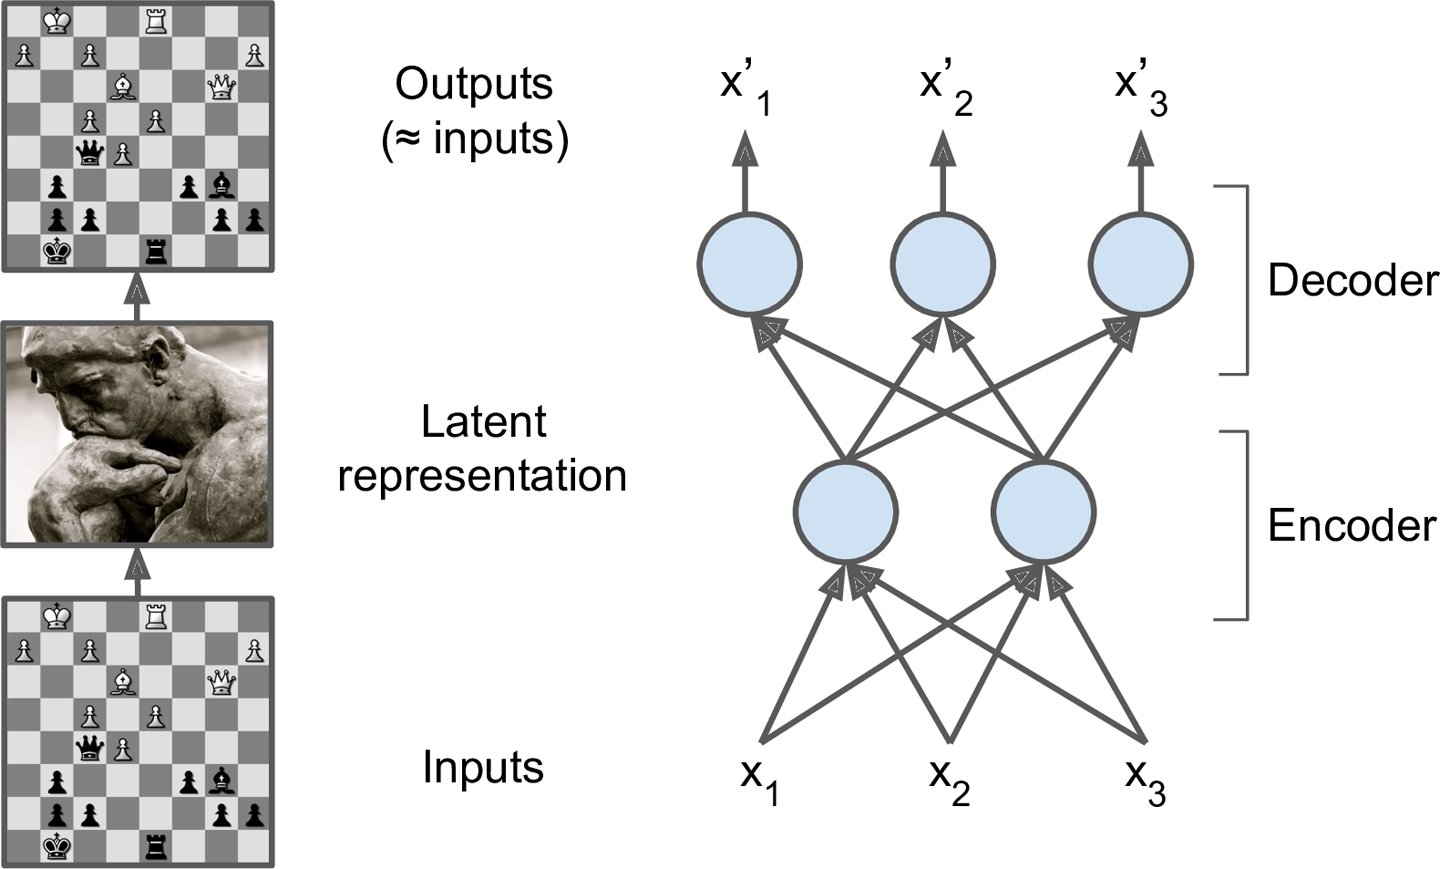
\includegraphics[width=0.5\textwidth]{./figure/ae}
\caption{The architecture of AE. Picture courtesy of \emph{Hands-On Machine Learning with Scikit-Learn, Keras, and TensorFlow (2nd Edition).}}\label{fig:ae}
\end{figure}
\vspace{-0.5cm}
\begin{itemize}
\footnotesize
\item As shown in fig.~\ref{fig:ae}, an AE has two parts:
	\begin{itemize}
	\footnotesize
	\item an \emph{Encoder} (a.k.a., \emph{Recognition Network}) that transforms the input into its latent representation
	\item an \emph{Decoder} (a.k.a., \emph{Generative Network}) that transforms the latent representation back to the input  
	\end{itemize}
\end{itemize}
\end{frame}

\begin{frame}
\setlength{\leftmargini}{0.3cm}
\setlength{\leftmarginii}{0.6cm}
\setlength{\leftmarginiii}{0.9cm}
\frametitle{The Architecture of Autoencoder}
\begin{figure}[h!]
\centering
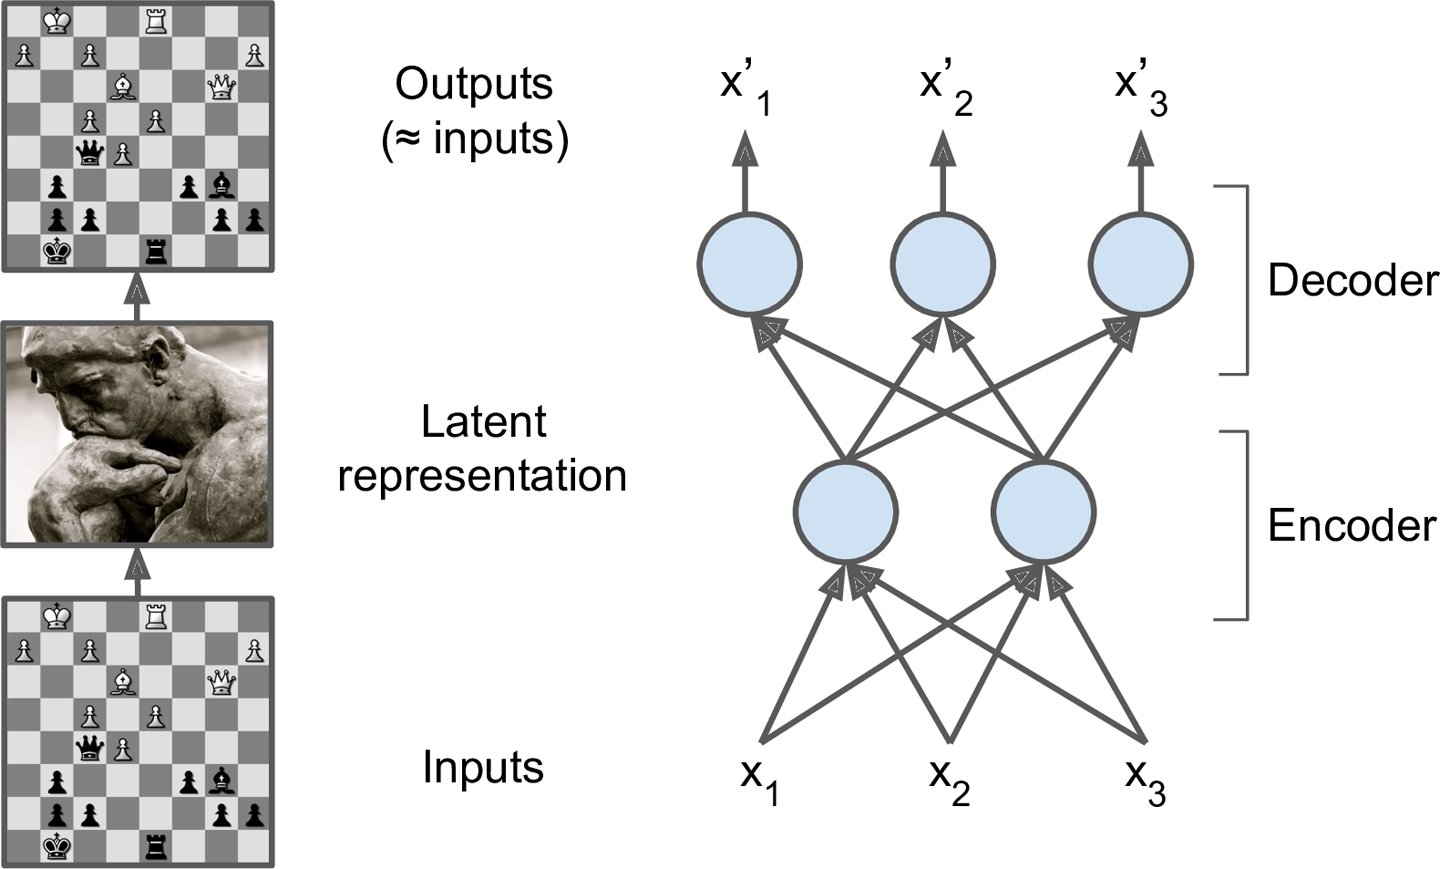
\includegraphics[width=0.5\textwidth]{./figure/ae}
\renewcommand\thefigure{1}
\addtocounter{figure}{-1}
\caption{The architecture of AE. Picture courtesy of \emph{Hands-On Machine Learning with Scikit-Learn, Keras, and TensorFlow (2nd Edition).}}
\end{figure}
\vspace{-0.5cm}
\begin{itemize}
\footnotesize
\item AE is essentially a Multi-Layer Perceptron (see \textcolor{blue}{\underline{\href{https://github.com/yuxiaohuang/teaching/blob/master/gwu/machine_learning_I/spring_2023/slides/p2_shallow_learning/p2_c2_supervised_learning/p2_c2_s4_shallow_neural_networks/shallow_neural_networks.pdf}{/p2\_c2\_s4\_shallow\_neural\_networks}}}):
	\begin{itemize}
	\footnotesize
	\item the encoder is the hidden layer
	\item the decoder is the output layer, where the number of perceptrons is the same as the number on the input layer (so as to reconstruct the input)
	\end{itemize}
\item AE reduces to Principal Component Analysis when:
	\begin{itemize}
	\footnotesize
	\item the activations are identity function
	\item the loss function is Mean Squared Error
	\end{itemize}
\end{itemize}
\end{frame}

\begin{frame}
\setlength{\leftmargini}{0.3cm}
\setlength{\leftmarginii}{0.6cm}
\setlength{\leftmarginiii}{0.9cm}
\frametitle{The Architecture of Stacked Autoencoder}
\begin{figure}[h!]
\centering
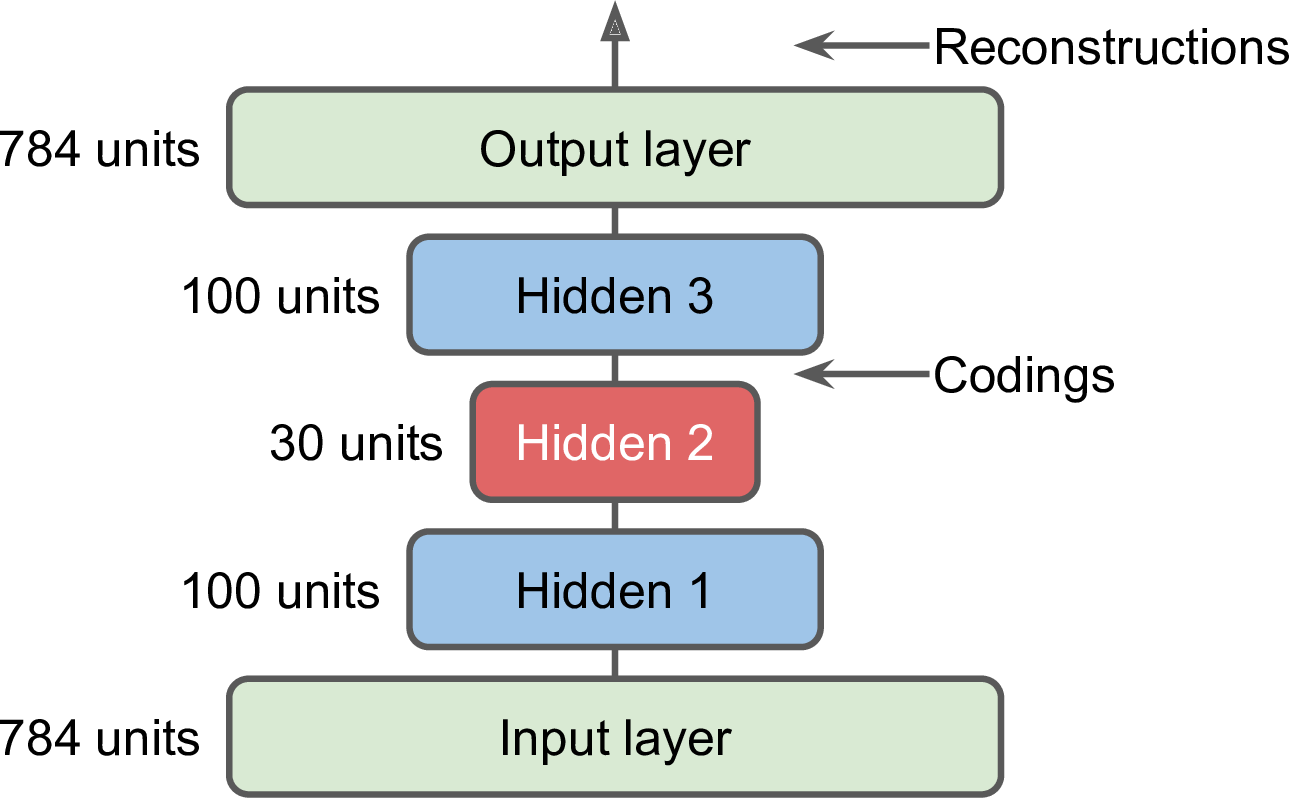
\includegraphics[width=0.5\textwidth]{./figure/sae}
\caption{The architecture of stacked AE. Picture courtesy of \emph{Hands-On Machine Learning with Scikit-Learn, Keras, and TensorFlow (2nd Edition).}}\label{fig:sae}
\end{figure}
\vspace{-0.5cm}
\begin{itemize}
\footnotesize
\item Similar to Multi-Layer Perceptron, we can add more hidden layers to AE to make it deep.
\item For an AE with multiple hidden layers, it is called \emph{Stacked Autoencoder} (Stacked AE).
\item As shown in fig.~\ref{fig:sae}, the architecture of stacked AE is typically symmetrical with regard to the central hidden layer (the coding layer). 
\end{itemize}
\end{frame}

\begin{frame}
\setlength{\leftmargini}{0.3cm}
\setlength{\leftmarginii}{0.6cm}
\setlength{\leftmarginiii}{0.9cm}
\frametitle{Transfer Learning with Stacked AE}
\begin{itemize}
\footnotesize
\item A key application of stacked AE is transfer learning.
\item The idea is that, for a large training set where most of the data are unlabeled, we can:
	\begin{enumerate}
	\footnotesize
	\item train a stacked AE on the whole (labeled and unlabeled) training data excluding the target (hence unsupervised learning)
	\item reuse the lower layers of the stacked AE as the base, and build a new model by adding layers on top of the base
	\item train the new model on the labeled training data (hence supervised learning):
		\begin{enumerate}
		\footnotesize
		\item first freeze (some or all) reused layers and only train the remaining layers
		\item unfreeze the frozen layers and train the whole model
		\end{enumerate} 
	\end{enumerate} 
\end{itemize}
\vspace{-0.2cm}
\begin{bclogo}
[couleur = green!30,
arrondi = 0,
%logo = \bccrayon,
ombre = false]
{Good practice}
\setlength{\leftmargini}{0.2cm}
\setlength{\leftmarginii}{0.2cm}
\begin{itemize}
\footnotesize
\item The steps for using stacked AE for transfer learning:
	\begin{enumerate}
	\footnotesize
	\item train a stacked AE on the whole (labeled and unlabeled) training data excluding the target (hence unsupervised learning)
	\item reuse the lower layers of the stacked AE as the base, and build a new model by adding layers on top of the base
	\item train the new model on the labeled training data (hence supervised learning):
		\begin{enumerate}
		\footnotesize
		\item first freeze (some or all) reused layers and only train the remaining layers
		\item unfreeze the frozen layers and train the whole model
		\end{enumerate} 
	\end{enumerate} 
\end{itemize}
\end{bclogo}
\end{frame}

%----------------------------------------------------------------------------------------
%	Variational Autoencoder
%----------------------------------------------------------------------------------------

\section{Variational Autoencoder}
\subsection{HML: Chap 17}
\begin{frame}
\setlength{\leftmargini}{0.3cm}
\setlength{\leftmarginii}{0.6cm}
\setlength{\leftmarginiii}{0.9cm}
\frametitle{The Architecture of Variational Autoencoder}
\begin{figure}[h!]
\centering
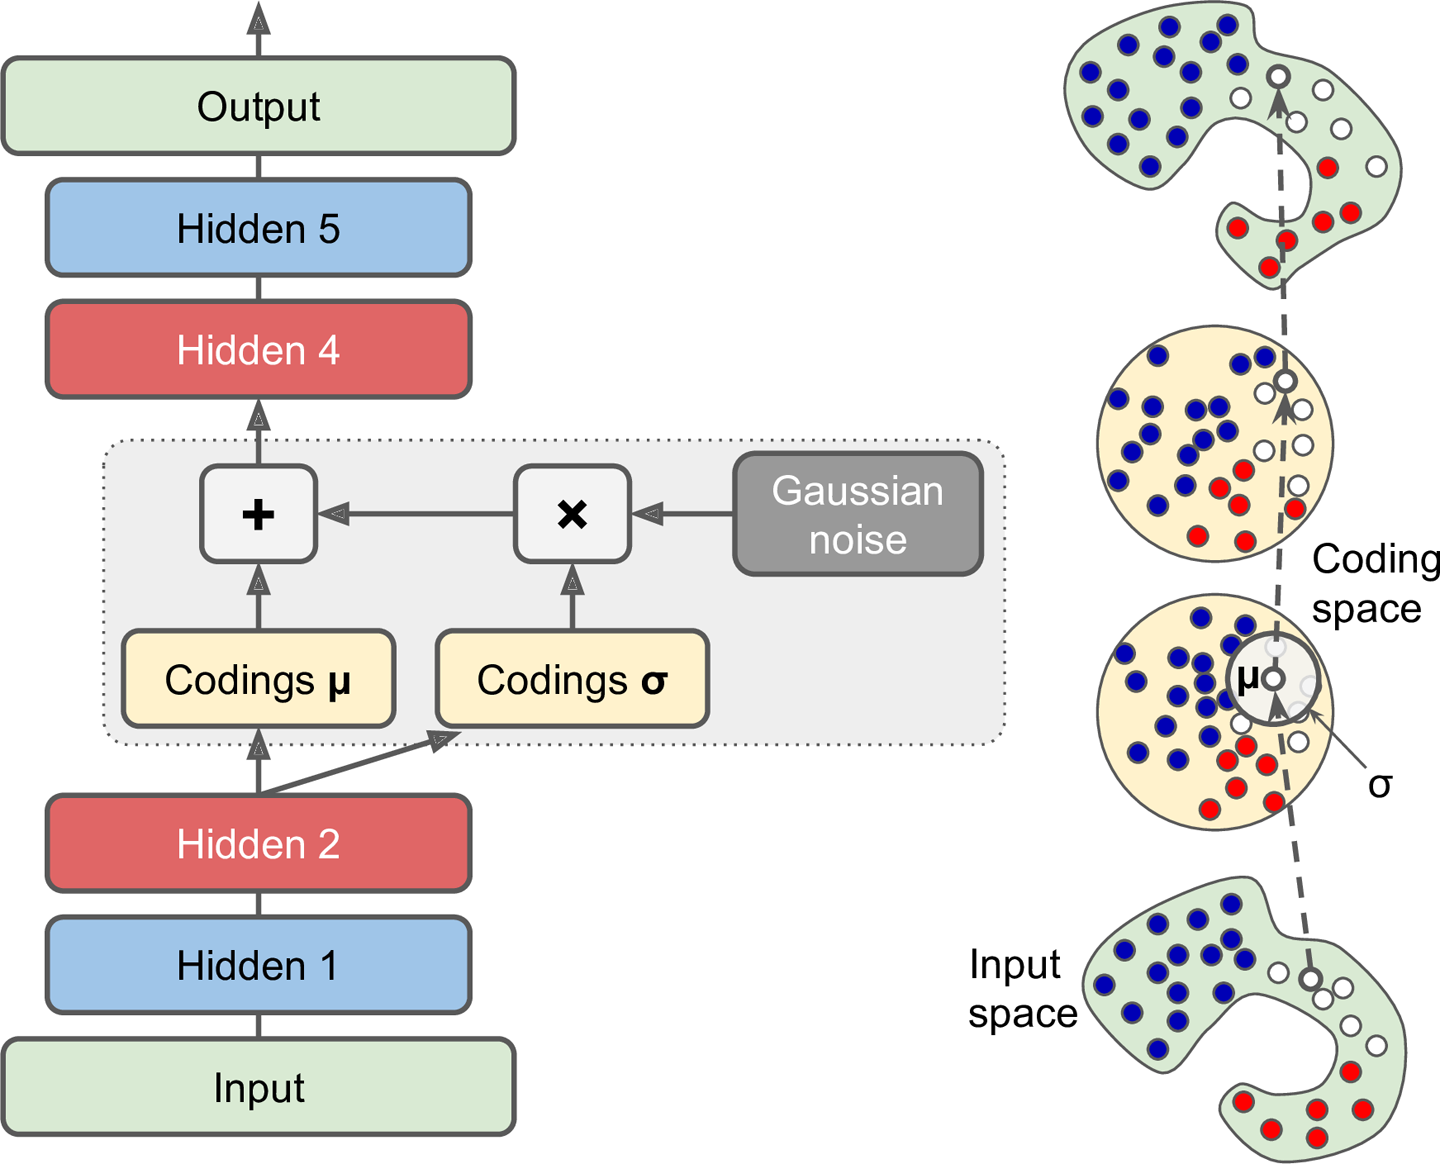
\includegraphics[width=0.4\textwidth]{./figure/vae}
\caption{The architecture of variational AE. Picture courtesy of \emph{Hands-On Machine Learning with Scikit-Learn, Keras, and TensorFlow (2nd Edition).}}\label{fig:vae}
\end{figure}
\vspace{-0.4cm}
\begin{itemize}
\footnotesize
\item A key extension of AE is \emph{Variational Autoencoder} (VAE).
\item The major differences between the architecture of AE and VAE are:
	\begin{itemize}
	\footnotesize
	\item the encoder in AE models the latent representation of the input
	\item the encoder in VAE models the latent representation of the mean ($\mu$) and standard deviation ($\sigma$) of a Gaussian distribution, which is the distribubtion of the latent representation of the input
	\end{itemize}
\end{itemize}
\end{frame}

\begin{frame}
\setlength{\leftmargini}{0.3cm}
\setlength{\leftmarginii}{0.6cm}
\setlength{\leftmarginiii}{0.9cm}
\frametitle{The Architecture of Variational Autoencoder}
\begin{figure}[h!]
\centering
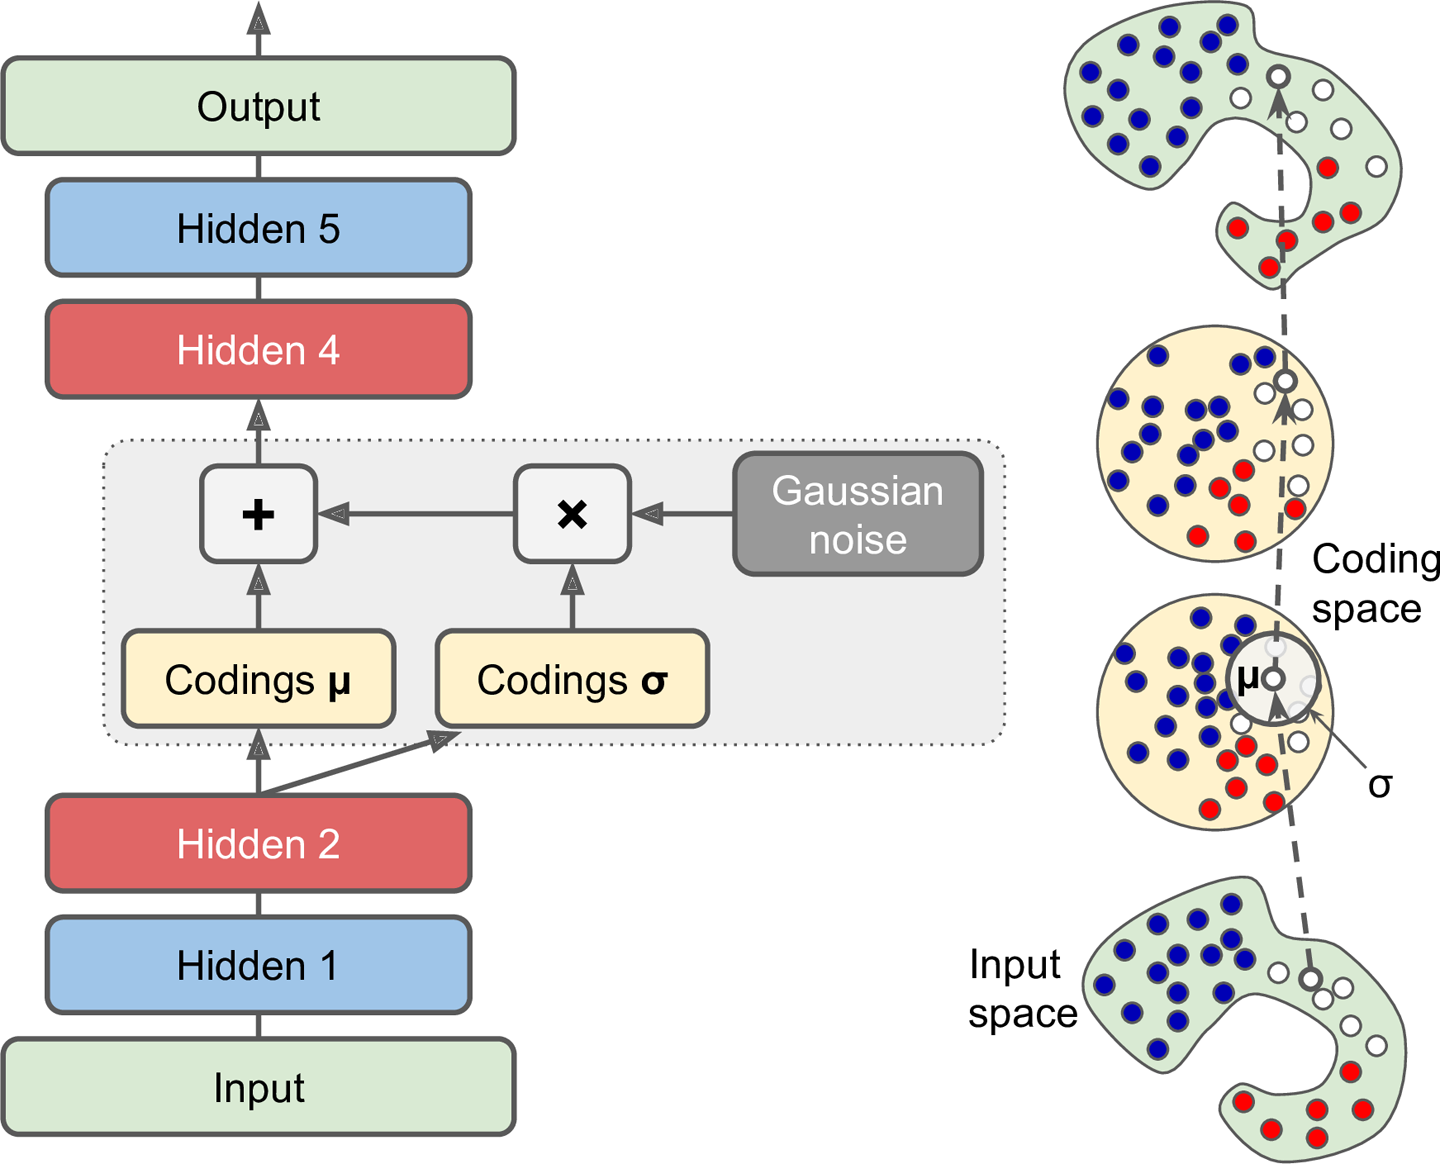
\includegraphics[width=0.4\textwidth]{./figure/vae}
\renewcommand\thefigure{3}
\addtocounter{figure}{-1}
\caption{The architecture of variational AE. Picture courtesy of \emph{Hands-On Machine Learning with Scikit-Learn, Keras, and TensorFlow (2nd Edition).}}
\end{figure}
\vspace{-0.4cm}
\begin{itemize}
\footnotesize
\item A key merit of VAE is that, after training we can generate new input by:
	\begin{itemize}
	\footnotesize
	\item sample the latent representation of the input from the Gaussian distribution
	\item decode the latent representation to generate new input
	\end{itemize} 
\item This also leads to another difference between AE and VAE:
	\begin{itemize}
	\footnotesize
	\item the output of AE is deterministic (as there is no randomness in AE's forward pass)
	\item the output of VAE is stochastic (as the latent representation of the input is sampled from a gaussian distribution)
	\end{itemize}
\end{itemize}
\end{frame}

%----------------------------------------------------------------------------------------
%	Generative Adversarial Networks
%----------------------------------------------------------------------------------------

\section{Generative Adversarial Networks}
\begin{frame}
\setlength{\leftmargini}{0.3cm}
\setlength{\leftmarginii}{0.6cm}
\setlength{\leftmarginiii}{0.9cm}
\frametitle{The Idea}
\begin{itemize}
\item Generative Adversarial Networks (GANs)~\cite{goodfellow2014generative} have received great attention for their good performance in generating artificial data resembling the real one. 
\item There are two components in GANs:
	\begin{itemize}
	\item a \emph{Generator} that tries to generate data similar to the real one
	\item a \emph{Discriminator} that tries to discriminate between the real data and the generated one
	\end{itemize}
\end{itemize}
\end{frame}

\begin{frame}
\setlength{\leftmargini}{0.3cm}
\setlength{\leftmarginii}{0.6cm}
\setlength{\leftmarginiii}{0.9cm}
\frametitle{The Idea}
\begin{itemize}
\item The idea of training GANs is based on an adversarial game  between the two components:
	\begin{itemize}
	\item the generator gets better (by deceiving the discriminator) only when the discriminator gets better (by debunking the generator)
	\item the discriminator gets better (by debunking the generator) only when the generator gets better (by deceiving the discriminator)
	\end{itemize}
\item In theory, as training advances GANs eventually reach a \emph{Nash Equilibrium} where:
	\begin{itemize}
	\item the generator generates data that perfectly mimic the real one
	\item the discriminator discriminates the two kinds of data with accuracy 0.5
	\end{itemize}
\end{itemize}
\end{frame}

\begin{frame}
\setlength{\leftmargini}{0.3cm}
\setlength{\leftmarginii}{0.6cm}
\setlength{\leftmarginiii}{0.9cm}
\frametitle{The Adversarial Game}
\begin{figure}[h!]
\centering
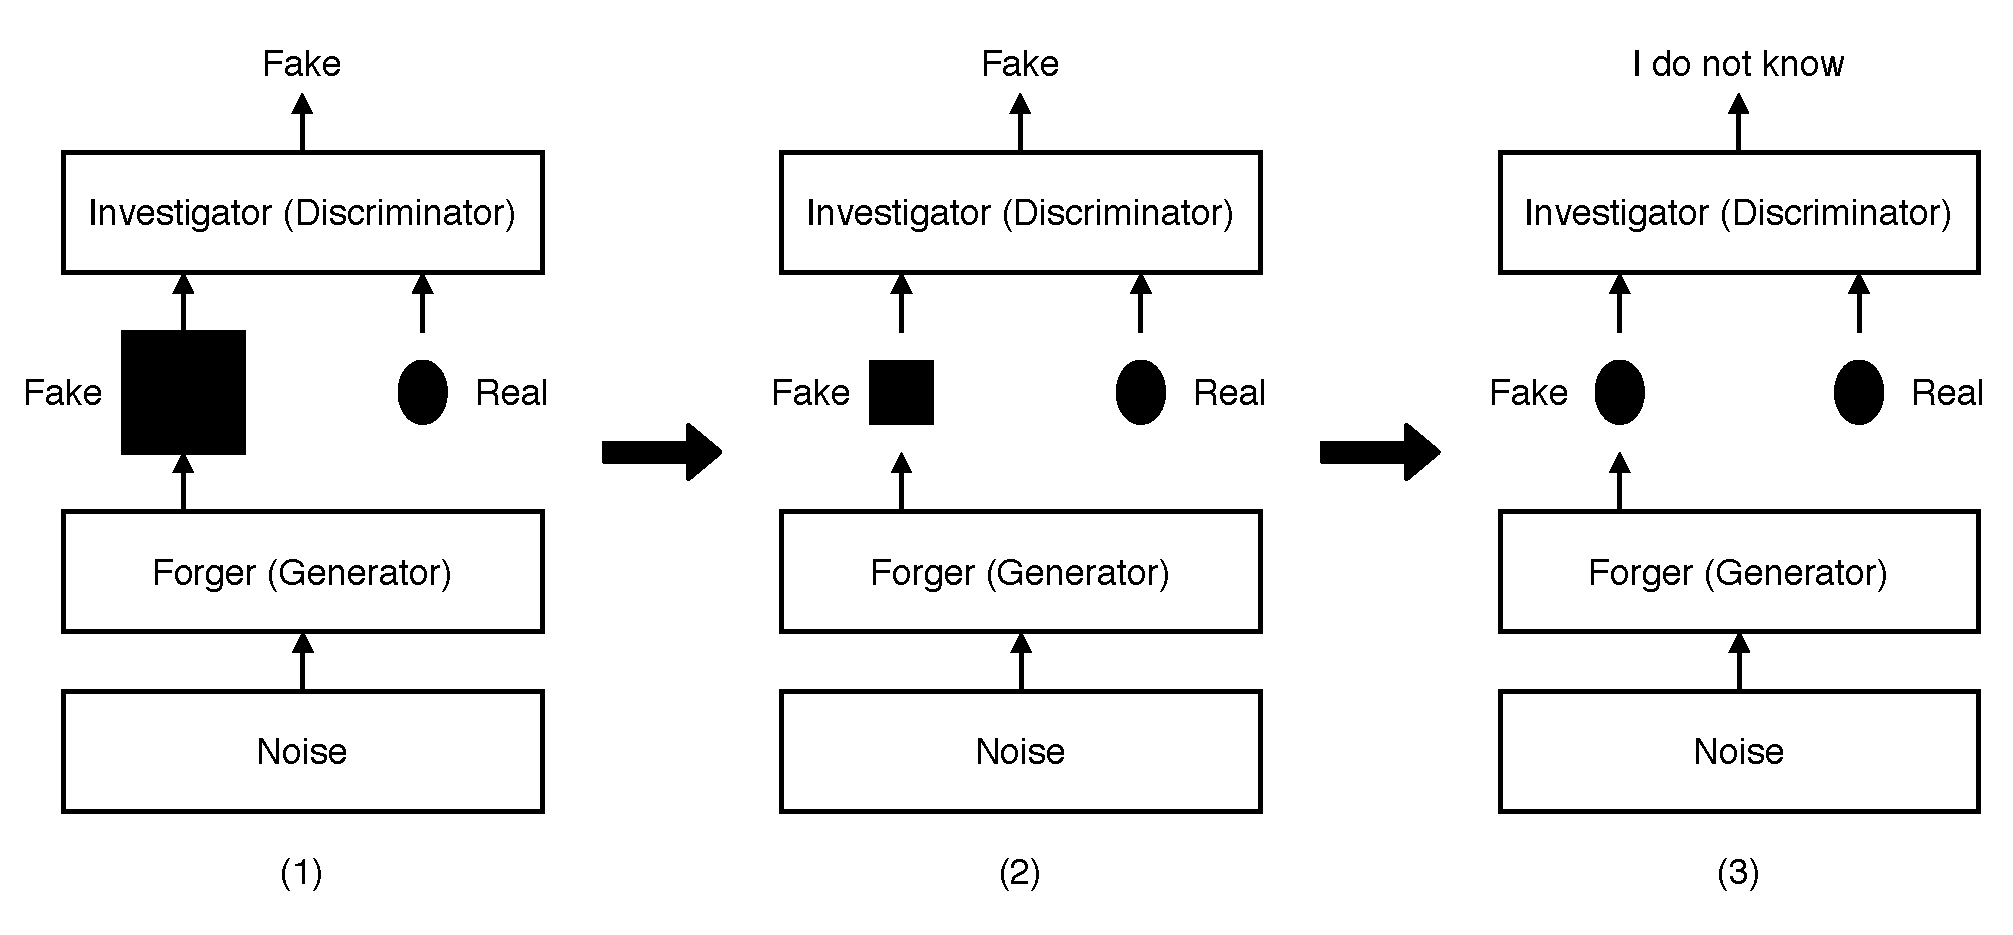
\includegraphics[width=1.0\textwidth]{./figure/gans}
\caption{\footnotesize{An example of the adversarial game between the generator and discriminator.}}\label{fig:gans}
\end{figure}
\end{frame}

\begin{frame}
\setlength{\leftmargini}{0.3cm}
\setlength{\leftmarginii}{0.6cm}
\setlength{\leftmarginiii}{0.9cm}
\frametitle{The Adversarial Game}
\begin{itemize}
\item Figure.~\ref{fig:gans} shows an example of the adversarial game between the generator and discriminator.
\item In this example, we use an adversarial game between a \emph{Forger} and an \emph{Investigator} to mimic the game between the generator and discriminator in GANs:
	\begin{itemize}
	\item a forger (generator) attempts to make fake pearls and sell them at a high price
	\item however, before selling them, the pearls have to be run by an investigator (discriminator), who decides whether the pearls are real
	\end{itemize}
\item Both the forger and investigator are in the early stage of their career, that is, neither of them is good at what they do:
	\begin{itemize}
	\item the forger makes big square-shaped pearls
	\item the investigator has no idea how to distinguish real pearls from fake ones
	\end{itemize}
\item The good news is, both of them are eager to learn. 
\end{itemize}
\end{frame}

\begin{frame}
\setlength{\leftmargini}{0.3cm}
\setlength{\leftmarginii}{0.6cm}
\setlength{\leftmarginiii}{0.9cm}
\frametitle{The Adversarial Game}
\begin{enumerate}
\footnotesize
\item The investigator learns by comparing the fake pearls with the real ones.
\item The first thing caught the investigator's eye is the size: real ones are small but fake ones are big. 
\item This insight was later leaked to the forger, he then starts making small square-shaped pearls to deceive the investigator.
\item This time, by comparing the fake pearls with the real ones, the investigator finds that he can also use the shape to separate the two kinds of pears: real ones are oval but fakes ones are square.
\item This insight was again leaked to the forger, he then starts making small oval-shaped pears to deceive the investigator.
\item By repeating this process, the investigator learns the differences between the real and fake pearls and the generator uses such information to narrow the differences. 
\item Eventually, the fake pearls are so perfect such that the discriminator cannot tell any difference anymore.
\end{enumerate}
\end{frame}

\begin{frame}
\setlength{\leftmargini}{0.3cm}
\setlength{\leftmarginii}{0.6cm}
\setlength{\leftmarginiii}{0.9cm}
\frametitle{The Loss Function}
\begin{itemize}
\footnotesize
\item The loss function of GANs, $V(\theta^{(D)}, \theta^{(G)})$, is
\begin{equation}\label{eq:loss_function}
E_{\mathbf{x}\sim p_{data}(\mathbf{x})}\left[\log D(\mathbf{x}) \right] + E_{\mathbf{z}\sim p_{\mathbf{z}}(\mathbf{z})}\left[\log \Big(1 - D \big(G(\mathbf{z}) \big) \Big) \right], \quad \textrm{where}
\end{equation}
\vspace{-0.5cm}
	\begin{itemize}
	\footnotesize
	\item $D$ is the discriminator
	\item $G$ is the generator
	\item $\mathbf{x}$ is the real data
	\item $\mathbf{z}$ is the latent vector and $G(\mathbf{z})$ the fake (generated) data
	\item $D(\mathbf{x})$ is the probability of $D$ correctly predicting $\mathbf{x}$ as real
	\item $D\big(G(\mathbf{z}) \big)$ is the probability of $D$ wrongly predicting $G(\mathbf{z})$ as real
	\item $E_{\mathbf{x}\sim p_{data}(\mathbf{x})}$ is the expectation with respect to the distribution of $\mathbf{x}$
	\item $E_{\mathbf{z}\sim p_{\mathbf{z}}(\mathbf{z})}$ is the expectation with respect to the distribution of $\mathbf{z}$
	\end{itemize}
\item In other words, the loss function is a sum of two expectations:
	\begin{itemize}
	\footnotesize
	\item the first expectation, $E_{\mathbf{x}\sim p_{data}(\mathbf{x})}$, is the average of the probability of the discriminator correctly predicting real data ($\mathbf{x}$ in eq.~\eqref{eq:loss_function}) as real
	\item the second expectation, $E_{\mathbf{z}\sim p_{\mathbf{z}}(\mathbf{z})}$, is the average of the probability of the discriminator correctly predicting fake data ($G(\mathbf{z})$ in eq.~\eqref{eq:loss_function}) as fake
	\end{itemize}
\item It is worth noting that while the discriminator is related to both expectations (to predict the data as real or fake), the generator is only related to the second expectation (to generate the fake data).
\end{itemize}
\end{frame}

\begin{frame}
\setlength{\leftmargini}{0.3cm}
\setlength{\leftmarginii}{0.6cm}
\setlength{\leftmarginiii}{0.9cm}
\frametitle{The Optimization}
\begin{itemize}
\item The optimization of GANs includes the following two steps (in order):
	\begin{enumerate}
	\item maximize the loss function, $V(\theta^{(D)}, \theta^{(G)})$, with respect to the discriminator, $D$
	\item minimize the loss function, $V(\theta^{(D)}, \theta^{(G)})$, with respect to the generator, $G$
	\end{enumerate}
\item The two steps above can be written as
\begin{equation}\label{eq:optimization}
\min_{G} \max_{D} V(\theta^{(D)}, \theta^{(G)}).
\end{equation}
\item At a glance, it is a bit strange that we optimize the loss using two completely opposite ways: 
	\begin{itemize}
	\item maximize it with respect to the discriminator
	\item minimize it with respect to the generator
	\end{itemize}
\item Here is why the optimization makes sense.
\end{itemize}
\end{frame}

\begin{frame}
\setlength{\leftmargini}{0.3cm}
\setlength{\leftmarginii}{0.6cm}
\setlength{\leftmarginiii}{0.9cm}
\frametitle{Maximization regarding the Discriminator}
\begin{itemize}
\item Eq.~\eqref{eq:loss_function} shows the loss function of GANs, $V(\theta^{(D)}, \theta^{(G)})$:
\begin{equation}
E_{\mathbf{x}\sim p_{data}(\mathbf{x})}\left[\log D(\mathbf{x}) \right] + E_{\mathbf{z}\sim p_{\mathbf{z}}(\mathbf{z})}\left[\log \Big(1 - D \big(G(\mathbf{z}) \big) \Big) \right].
\tag{\ref{eq:loss_function}}
\end{equation}
\item In the first expectation of the loss, $D(\mathbf{x})$ is the probability of the discriminator correctly predicting the real data, $\mathbf{x}$, as real.
\item The discriminator wants this probability as close to 1 (the maximum value of a probability) as possible, as 1 means the discriminator is certain that the real data is real.
\item Since $\log D(\mathbf{x})$ is strictly increasing (i.e., the higher $D(\mathbf{x})$ the higher $\log D(\mathbf{x})$), making $D(\mathbf{x})$ as large as possible equates making $\log D(\mathbf{x})$ as large as possible, hence maximizing the first expectation.
\end{itemize}
\end{frame}

\begin{frame}
\setlength{\leftmargini}{0.3cm}
\setlength{\leftmarginii}{0.6cm}
\setlength{\leftmarginiii}{0.9cm}
\frametitle{Maximization regarding the Discriminator}
\begin{itemize}
\item Eq.~\eqref{eq:loss_function} shows the loss function of GANs, $V(\theta^{(D)}, \theta^{(G)})$:
\begin{equation}
E_{\mathbf{x}\sim p_{data}(\mathbf{x})}\left[\log D(\mathbf{x}) \right] + E_{\mathbf{z}\sim p_{\mathbf{z}}(\mathbf{z})}\left[\log \Big(1 - D \big(G(\mathbf{z}) \big) \Big) \right].
\tag{\ref{eq:loss_function}}
\end{equation}
\item In the second expectation of the loss, $D\big(G(\mathbf{z}) \big)$ is the probability of the discriminator wrongly predicting the fake data, $G(\mathbf{z})$, as real.
\item The discriminator wants this probability as close to 0 (the minimum value of a probability) as possible, as 0 means the discriminator is certain that the fake data is not real.
\item Since $\log \Big(1 - D \big(G(\mathbf{z}) \Big)$ is strictly increasing (i.e., the higher $1 - D \big(G(\mathbf{z})$ the higher $\log \Big(1 - D \big(G(\mathbf{z}) \Big)$), making $D\big(G(\mathbf{z}) \big)$ as small as possible equates making $1 - D \big(G(\mathbf{z})$ as large as possible, which in turn, equates making $\log \Big(1 - D \big(G(\mathbf{z}) \Big)$ as large as possible, hence maximizing the second expectation.
\end{itemize}
\end{frame}

\begin{frame}
\setlength{\leftmargini}{0.3cm}
\setlength{\leftmarginii}{0.6cm}
\setlength{\leftmarginiii}{0.9cm}
\frametitle{Maximization regarding the Discriminator}
\begin{itemize}
\item To sum up, since we want to maximize both the first and the second expectation in the loss function, we want to maximize the whole loss function with respect to the discriminator.
\item This is why we have the maximization in eq.~\eqref{eq:optimization}
\begin{equation}
\min_{G} \max_{D} V(\theta^{(D)}, \theta^{(G)}).
\tag{\ref{eq:optimization}}
\end{equation}
\end{itemize}
\end{frame}

\begin{frame}
\setlength{\leftmargini}{0.3cm}
\setlength{\leftmarginii}{0.6cm}
\setlength{\leftmarginiii}{0.9cm}
\frametitle{Minimization regarding the Generator}
\begin{itemize}
\footnotesize
\item Eq.~\eqref{eq:loss_function} shows the loss function of GANs, $V(\theta^{(D)}, \theta^{(G)})$:
\begin{equation}
E_{\mathbf{x}\sim p_{data}(\mathbf{x})}\left[\log D(\mathbf{x}) \right] + E_{\mathbf{z}\sim p_{\mathbf{z}}(\mathbf{z})}\left[\log \Big(1 - D \big(G(\mathbf{z}) \big) \Big) \right].
\tag{\ref{eq:loss_function}}
\end{equation}
\item Since only the second expectation in the loss is related to the generator, we only need to discuss why we should minimize the second expectation with respect to the generator.
\item As mentioned earlier, in the second expectation $D\big(G(\mathbf{z}) \big)$ is the probability of the discriminator wrongly predicting the fake data, $G(\mathbf{z})$, as real.
\item The generator wants this probability as close to 1 as possible, as 1 means that the discriminator is certain that the fake data is real.
\item Since $\log \Big(1 - D \big(G(\mathbf{z}) \Big)$ is strictly increasing, making $D\big(G(\mathbf{z}) \big)$ as large as possible equates making $1 - D \big(G(\mathbf{z})\big)$ as small as possible, hence minimizing the second expectation.
\item This is why we have the minimization in eq.~\eqref{eq:optimization}
\begin{equation}
\min_{G} \max_{D} V(\theta^{(D)}, \theta^{(G)}).
\tag{\ref{eq:optimization}}
\end{equation}
\end{itemize}
\end{frame}

\begin{frame}
\setlength{\leftmargini}{0.3cm}
\setlength{\leftmarginii}{0.6cm}
\setlength{\leftmarginiii}{0.9cm}
\frametitle{Training GANs}
\begin{itemize}
\item A practical way of training GANs is to alternate between the two optimization steps (in order):
	\begin{enumerate}
	\item freeze the parameters of the generator and update the parameters of the discriminator
	\item freeze the parameters of the discriminator and update the parameters of the generator
	\end{enumerate}
\end{itemize}
\end{frame}

\subsection{PML: Chap 17}
\begin{frame}
\setlength{\leftmargini}{0.3cm}
\setlength{\leftmarginii}{0.6cm}
\setlength{\leftmarginiii}{0.9cm}
\frametitle{Training GANs}
\begin{figure}[h!]
\centering
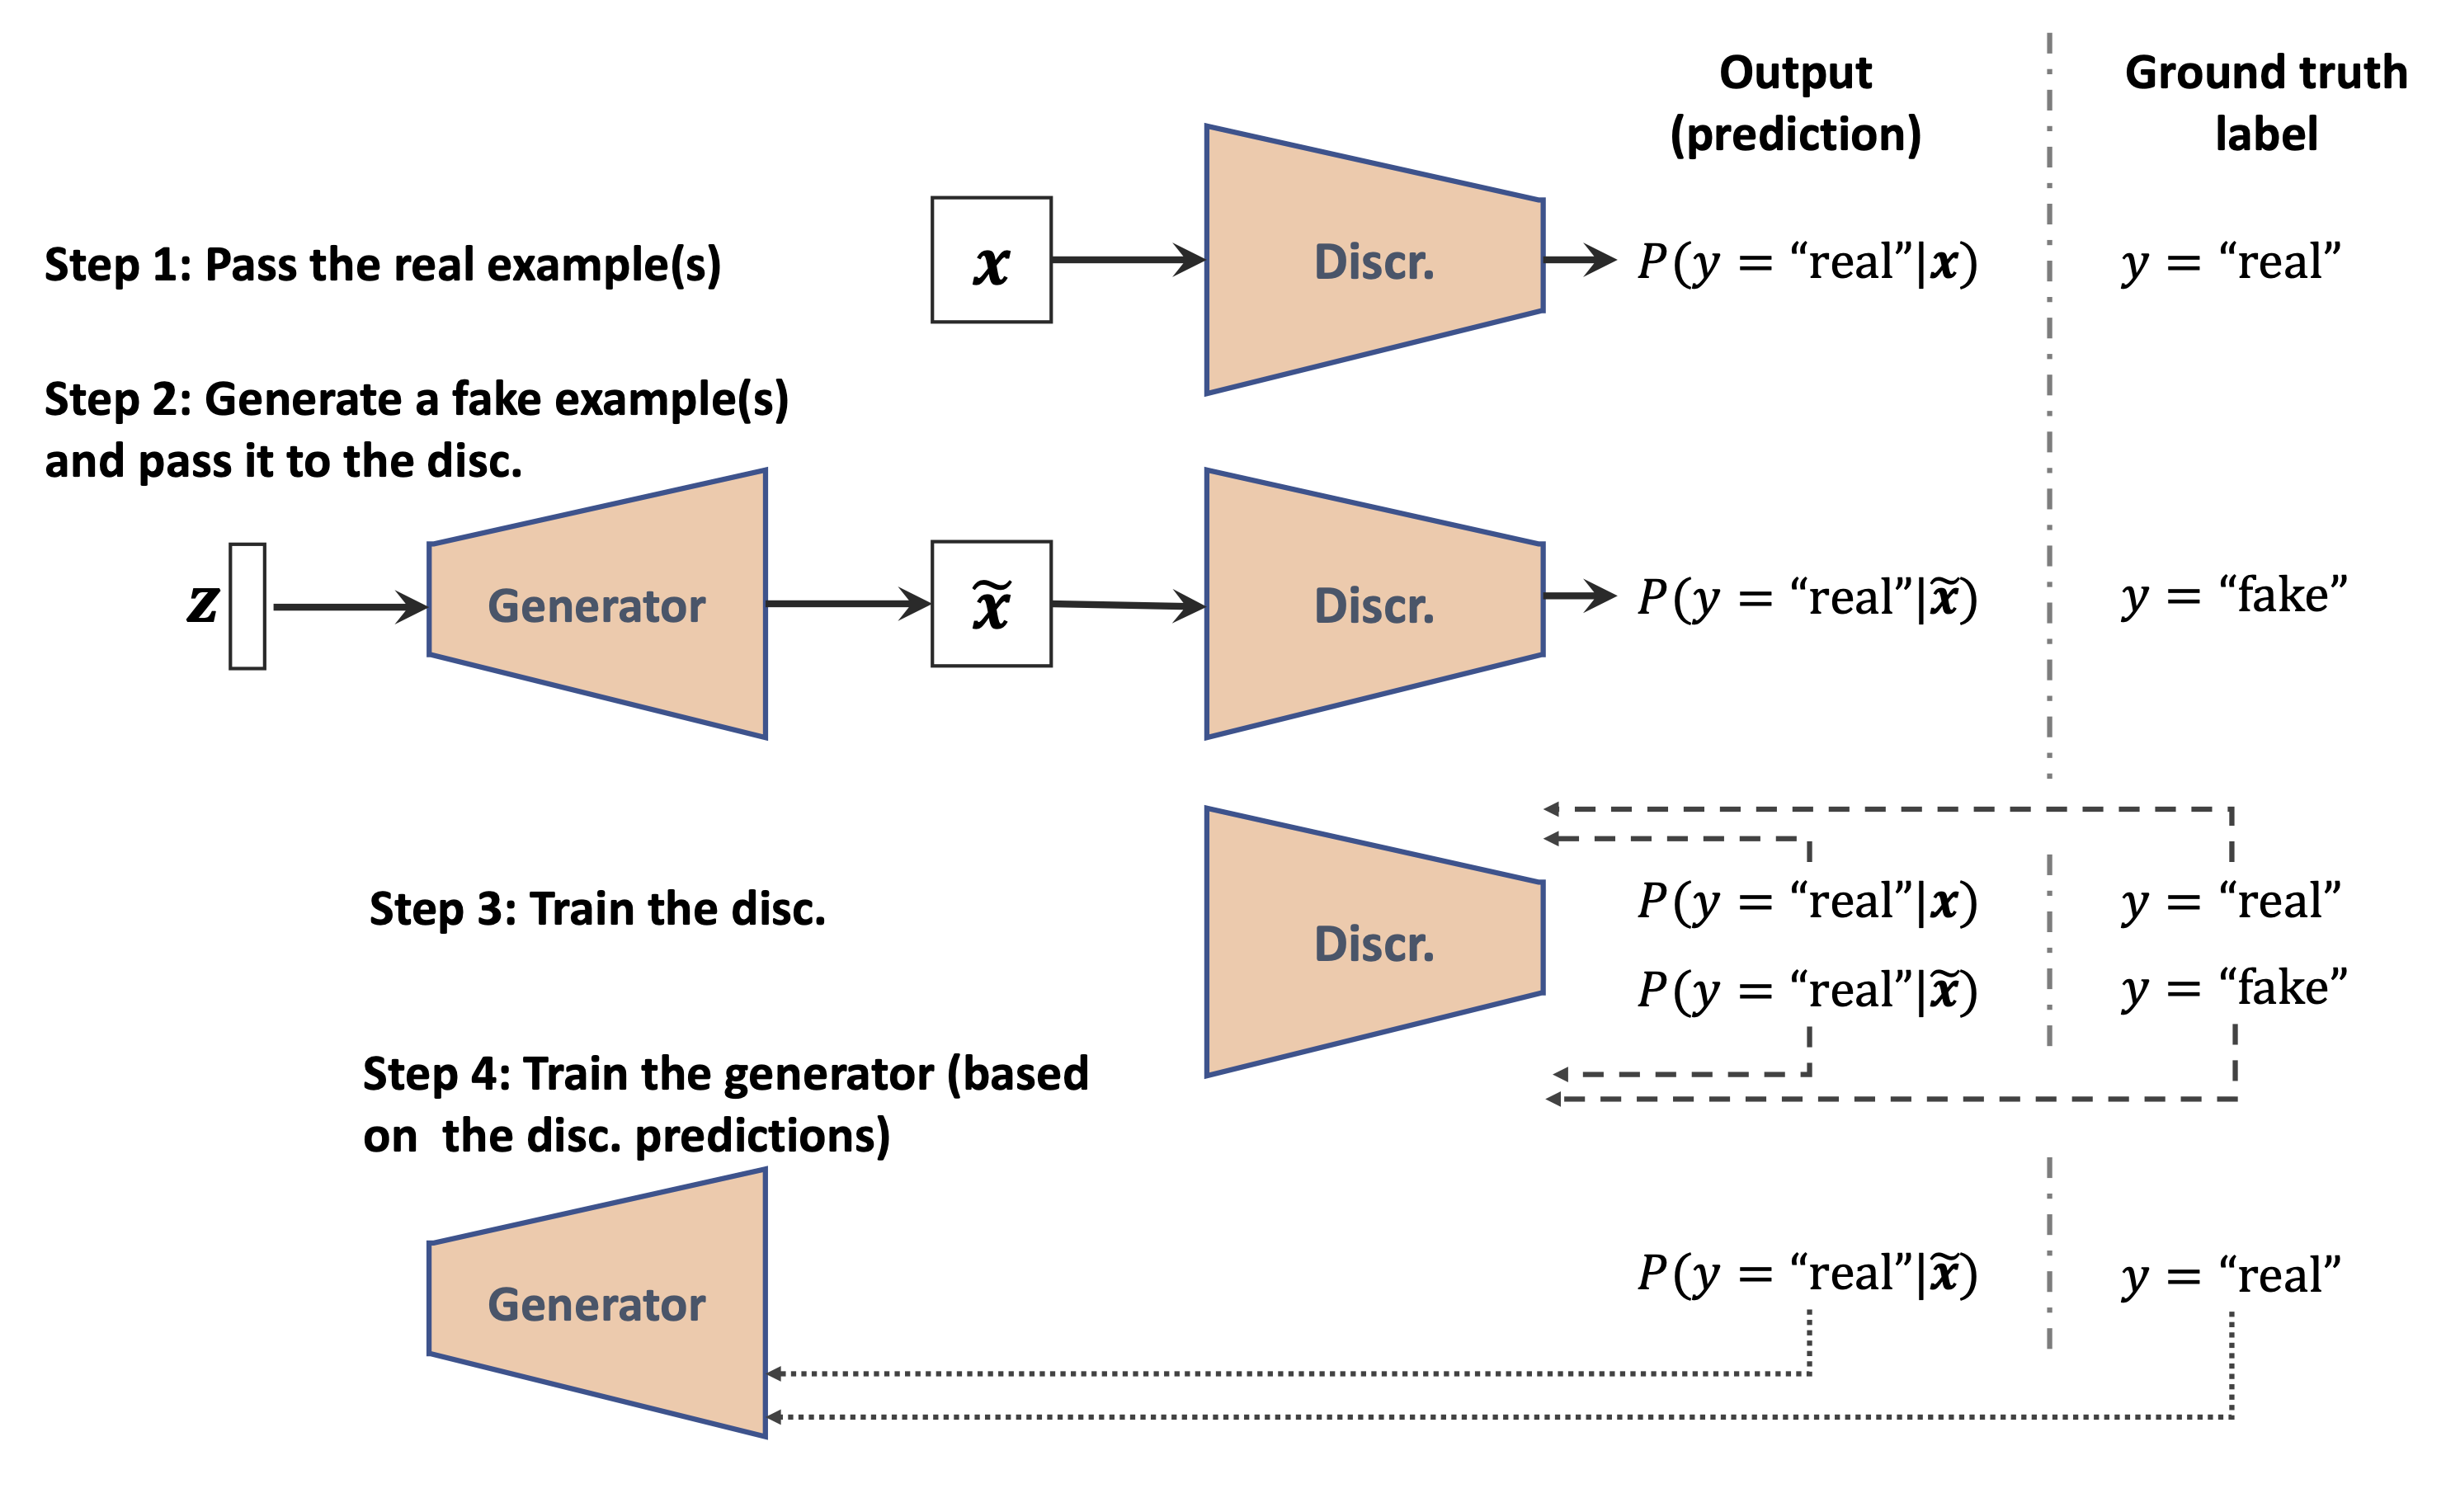
\includegraphics[width=0.8\textwidth]{./figure/training_gan}
\caption{\footnotesize{One iteration of training GANs. Picture courtesy of \emph{Python Machine Learning (3rd Edition).}}}
\label{fig:training_gan}
\end{figure}
\end{frame}

\subsection{HML: Chap 17}
\begin{frame}
\setlength{\leftmargini}{0.3cm}
\setlength{\leftmarginii}{0.6cm}
\setlength{\leftmarginiii}{0.9cm}
\frametitle{Deep Convolutional GANs}
\begin{itemize}
\item GANs based on deep CNNs have been proposed to generate large images.
\item One popular model is Deep Convolutional GANs (DCGANs)~\cite{radford2015unsupervised}.
\end{itemize}
\vspace{-0.4cm}
\begin{bclogo}
[couleur = green!30,
arrondi = 0,
%logo = \bccrayon,
ombre = false]
{Good practice}
\setlength{\leftmargini}{0.2cm}
\setlength{\leftmarginii}{0.2cm}
\begin{itemize}
\item Follow the following good practices to build stable DCGANs:
	\begin{itemize}
	\item replace any pooling layer with strided convolutions (in the discriminator) and transposed convolutions (in the generator)
	\item use \emph{Batch Normalization} in both the generator and the discriminator, except in the generator's output layer and discriminator's input layer
	\item remove fully connected hidden layers
	\item use \texttt{ReLU} activation in the generator for all layers except the output layer, which should use tanh
	\item use \texttt{leaky ReLU} activation in the discriminator for all layers
	\end{itemize}
\end{itemize}
\end{bclogo}
\end{frame}

\subsection{}
\begin{frame}
\setlength{\leftmargini}{0.3cm}
\setlength{\leftmarginii}{0.6cm}
\setlength{\leftmarginiii}{0.9cm}
\frametitle{Further Reading}
\begin{itemize}
\item See a detailed discussion of GAN in a NeurlPS 2016 tutorial:
\textcolor{blue}{\underline{\url{https://arxiv.org/pdf/1701.00160.pdf}}}
\item See an important improvement of GAN, Wasserstein GAN (WGAN), in:
\textcolor{blue}{\underline{\url{https://arxiv.org/pdf/1701.07875.pdf}}}
\item See an important improvement of WGAN in:
\textcolor{blue}{\underline{\url{https://arxiv.org/pdf/1704.00028.pdf}}}
\end{itemize}
\end{frame}

%\begin{frame}
\setlength{\leftmargini}{0.3cm}
\setlength{\leftmarginii}{0.6cm}
\setlength{\leftmarginiii}{0.9cm}
%\frametitle{Popular RNNs and Their Applications in NLP}
%\begin{itemize}
%\item In this section we will introduce some popular RNNs and their applications in NLP:
%	\begin{itemize}
%	\item Character RNN for Text Generation
%	\item Encoder-Decoder for Neural Machine Translation
%	\item Attention Mechanisms
%	\end{itemize}
%\end{itemize}
%\end{frame}

%----------------------------------------------------------------------------------------
%	Bibliography
%%----------------------------------------------------------------------------------------

\section{Bibliography}
\begin{frame}[t,allowframebreaks]
\setlength{\leftmargini}{0.3cm}
\setlength{\leftmarginii}{0.6cm}
\setlength{\leftmarginiii}{0.9cm}
\frametitle{Bibliography}
\footnotesize
\bibliographystyle{apalike}
\bibliography{references}
\end{frame}

\end{document} 